\section{Présentation de Elasticsearch}


\section{Installation}
Avant même de regarder les différentes dépendances nécessaires à l'utilisation de
elasticsearch il est recommandé devérifier que l'on utilise bien la même version
que son compère logstash (vérifier la documentation).

Son installation est sensiblement la même que son comparse logstash puisque ce logiciel 
nécessite également l'installation des dépendances \emph{jruby} et \emph{openjdk-7-jre}
à noter qu'il fonctionne également sur openjdk-8-jre.

Là aussi les paquets debian officiels n'existant pas on utilisera celui fourni par 
elastic.co\footnote{https://download.elastic.co/elasticsearch/elasticsearch/elasticsearch-1.5.1.deb}.
Et ici aussi le paquet est un peu approximatif puisqu'il faut rajouter certains chemin, et ajouter des droits.




Acompleter et revoir
p24-26
 test


\section{Sense}
Sense est un module chrome développé par Boaz Leskes, il sert de front-end à ElasticSearch.
Le développement (public) de ce module est maintenant arrêté. Il fait parti de 
\emph{Marvel} le logiciel de monitoring et d'optimisation, vendu\footnote{voir bas 
de page : \url{https://www.elastic.co/products/marvel/signup.html}} 
par la société \emph{elastic}.


\subsection{Installation}
Installer ce logiciel est simple comme installer une extension Chrome\footnote{testé sur chromium}
tierce.
Tout d'abord : récupérer le module à l'agresse  https://github.com/bleskes/sense 
en utilisant par exemple : 
\begin{lstlisting}[style=code]
git clone https://github.com/bleskes/sense.git
\end{lstlisting}

Il suffit ensuite de l'activer dans chromium :\\ 
chrome://extension => Developer mode => Load unpacked extension.

\begin{figure}
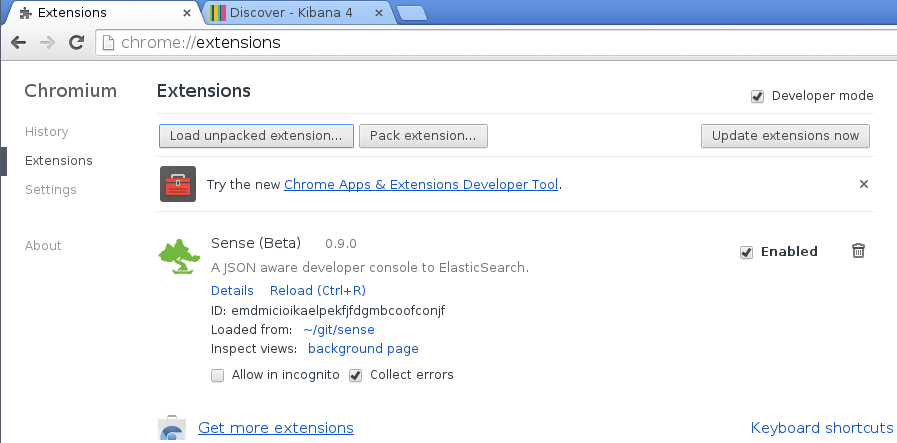
\includegraphics{senseinstall.png}
\label{fig:senseinstall}
\caption Plugin Sense installé dans chromium
\end{figure}

Et voilà !

\subsection{Utilisation de Sense}
